\chapter{Teknisk beskrivelse}

\section{Databaseabstraktion}

I parallel med Bookie har vi udviklet en databaseabstraktion ved navn \textit{Donkey}. Donkey er bygget oven på JDBC (Java Database Connectivity) og har til formål at muliggøre persistens af datamodeller uden at en udvikler behøver skrive en eneste linje SQL. Dette opnås gennem såkaldt \textit{object-relational mapping} (forkortet \textit{ORM}), hvor et objekt i et objekt-orienteret system–i vores tilfælde Java–automatisk kan konverteres til en mere simpel struktur, som kan gemmes i et databasesystem (\cite{wiki:orm}).

Donkey understøtter på nuværende tidspunkt tre forskellige relationelle databasesystemer: MySQL\footnote{\url{http://www.mysql.com/}}, PostgreSQL\footnote{\url{http://www.postgresql.org/}}, samt SQLite\footnote{\url{http://sqlite.org/}}. Mens Bookie udelukkende gør brug af SQLite, er understøttelse af de resterende databasesystemer medtaget for at sikre en solid løsning, som kan tage forbehold for eventuelle forskelle mellem databasesystemer.

Donkeys grundlæggende byggedele er baserede på Laravels\footnote{\url{http://laravel.com/}} API'er, da disse allerede var en af forfatterne kendte. Konceptuelt låner Donkey begreberne om \textit{Grammars}, \textit{Queries}, samt \textit{Schemas} og benytter disse til at implementere ORM i form af \textit{Models}. En datamodel i Donkey er i sidste ende derfor ikke andet end en klasse, som repræsenterer en tabel i en relationsdatabase, og en række offentlige felter i denne klasse, som repræsenterer tabellens kolonner og datatyperne af disse. Dette er igen relateret til Laravel og dens \textit{Eloquent ORM}\footnote{\url{http://laravel.com/docs/4.2/eloquent}} dog med den forskel, at Donkeys implementation af ORM endnu ikke er nær så fleksibel som Laravels.

Helt konkret består Donkey af følgende klasser:

\begin{multicols}{3}
\begin{itemize}
  \item \texttt{Grammar}
    \begin{itemize}
      \item \texttt{MySqlGrammar}
      \item \texttt{PostgreSqlGrammar}
      \item \texttt{SqliteGrammar}
    \end{itemize}
  \item \texttt{Driver}
  \item \texttt{Row}
  \item \texttt{Database}
  \item \texttt{Query}
  \item \texttt{Schema}
  \item \texttt{Model}
  \item \texttt{ModelQuery}
\end{itemize}
\end{multicols}

Donkey er fra bunden opbygget efter \textit{dependency injection} designmønstret, hvor afhængigheder injiceres i afhængende klasser frem for selv at lade de afhængende klasser finde og instantiere deres afhængigheder (\cite{wiki:di}). Dette designmønster har vi fulgt, da det gav større kontrol over, hvorledes afhængigheder flød igennem systemet. Eftersom \texttt{Grammar}-klassen er en afhængighed i næsten samtlige andre klasser (mere om dette følger), og da \texttt{Grammar} er abstrakt med de konkerete implementationer \texttt{MySqlGrammar}, \texttt{PostgreSqlGrammar}, og \texttt{SqliteGrammar}, ville det have været yderst besværligt at opbygge systemet, hvis ikke denne grundlæggende afhængighed kunne injiceres i de afhængende klasser. Figur \ref{class-diagram:database-abstraction} forsøger at tydeliggøre, hvorledes de forskellige afhængigheder flyder gennem systemet samt hvordan disse injiceres i de afhængende klasser.

\begin{figure}[h]
  \centering
  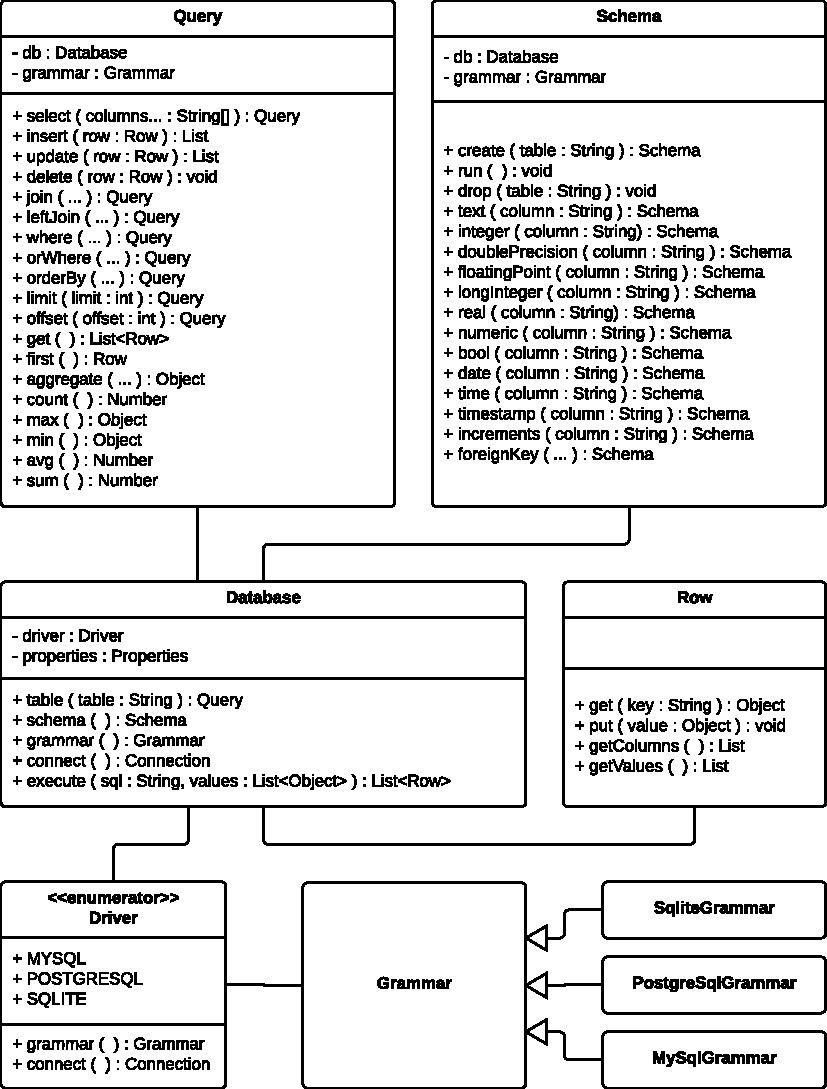
\includegraphics[scale=0.75]{database-abstraction.pdf}
  \caption{Lettere forsimplet klassediagram over databaseabstraktionen, ORM ekskluderet.}
  \label{class-diagram:database-abstraction}
\end{figure}

De næste sektioner vil gennemgå hver klasse i det niveau af detalje, som måtte være sig passende for den enkelte klasse.

\subsection{Row}

\texttt{Row}-klassen er en subklasse af \texttt{LinkedHashMap} og beskriver en datastruktur, der benyttes til at opbevare databaserækker. Den er fundamental for resten af systemet, idet den er bindeledet mellem Donkeys klasser og JDBCs \texttt{ResultSet}\footnote{\url{https://docs.oracle.com/javase/8/docs/api/java/sql/ResultSet.html}}-strukturer, som bruges til at opbevare tabeller af data resulterende fra databaseforespørgsler.

\texttt{Row}-klassen benytter sig af de generiske typer \texttt{String} og \texttt{Object} til nøgler og værdier, respektivt, i et \texttt{LinkedHashMap}. Dette gør det muligt at associere en databasekolonne (nøglen) med en hvilken som helst datatype (værdien), hvilket er hensigtmæssigt, da en databasetabel kan indeholde mange forskellige typer af data.

Slutteligt bør det nævnes, at et \texttt{LinkedHashMap} blev valgt, da iterationsrækkefølgen af kolonnerne i en tabel i visse tilfælde \textit{kan} have betydning.

\subsection{Grammar}

Den abstrakte \texttt{Grammar}-klasse benyttes til at bygge de forskellige delkomponenter af SQL-udtryk samt til at kompilere disse delkomponenter til fulde SQL-udtryk. Som navnet på klassen indikerer, bruges den dermed til at beskrive grammatikken for SQL-udtryk:

\begin{figure}[h]
  \begin{minted}{java}
  Grammar g = new FooGrammar();

  g.addTable("table");
  g.addColumn("col1");
  g.addColumn("col2");
  g.addWhere("col1", ">", 123, "and");
  g.addWhere("col2", "=", "bar", "or");
  
  g.compileSelect();
  // => "select col1, col2 from table where col1 > ? or col2 = ?"
  \end{minted}
  \caption{Eksempel på kompilering af et \texttt{select}-udtryk via \texttt{Grammar}}
  \label{code-example:grammar-select-compilation}
\end{figure}

\begin{wrapfigure}{r}{0.35\textwidth}
  \centering
  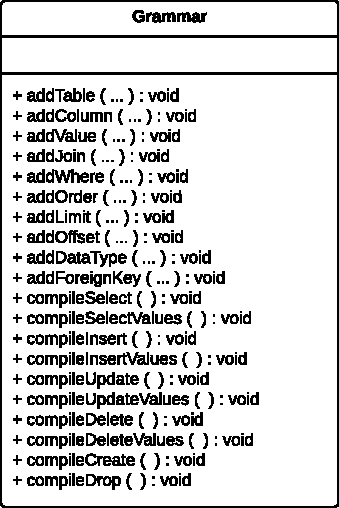
\includegraphics[width=0.275\textwidth]{grammar-class.pdf}
  \caption{Klassediagram for \texttt{Grammar}}
  \label{class-diagram:grammar-class}
\end{wrapfigure}

Læg i figur \ref{code-example:grammar-select-compilation} specielt mærke til hvorledes værdierne \texttt{123} og \texttt{"bar"} bliver erstattede med \texttt{?} i det kompilerede SQL-udtryk. Hvorfor dette gøres, vil vi komme tilbage til senere.

Målet med \texttt{Grammar}-klassen er at definere en grammatik for de mest typiske og standardiserede SQL-udtryk. Klassen er imidlertid abstrakt, da ikke alle understøttede SQL-udtryk er standardiserede mellem de forskellige databasesystemer. Dette inkluderer på nuværende tidspunkt definitionen af automatisk stigende kolonner, hvilket ikke håndteres ens mellem de understøttede databasesystemer. \texttt{Grammar} definerer derfor dette stykke funktionalitet som en abstrakt metode, der overlades til underklasser at implementere.

Figur \ref{class-diagram:grammar-class} viser de vigtigste offentlige metoder tilgængelige i \texttt{Grammar}-klassen. Alle metodeparametre er fjernede, da disse ikke umiddelbart har betydning for at danne et billede af den overordnede funktionalitet tilgængelig i \texttt{Grammar}. Med denne funktionalitet, omend lidt sparsommelig, er det muligt at dække de hyppigst forekommende SQL-udtryk, i hvert fald i det omfang vi vil benytte i Bookie.

\subsection{Driver}

\texttt{Driver}-enumeratoren har til opgave at oprette forbindelse til de understøttede databasesystemer via JDBCs \texttt{DriverManager}\footnote{\url{http://docs.oracle.com/javase/8/docs/api/java/sql/DriverManager.html}} og de tredjepartsdrivere, som måtte være tilgængelige for det pågældende databasesystem. Derudover står \texttt{Driver}-enumeratoren også for at instantiere de konkrete \texttt{Grammar}-objekter, som skal benyttes til de forskellige databasesystemer. MySQL-driveren opretter dermed instanser af \texttt{MySqlGrammar}, PostgreSQL-driveren instanser af \texttt{PostgreSqlGrammar}, og slutteligt SQLite-driveren instanser af \texttt{SqliteGrammar}.

\texttt{Driver} er implementeret som en enumerator og ikke en klasse, da vi ikke så mening i at have et interface med tre implementerende klasser hver med kun to statiske metoder. En enumerator med to abstrakte metoder, som implementeres i hver af enumratorens elementer, var derfor at foretrække.

Der henvises til figur \ref{class-diagram:database-abstraction} for klassediagrammet for \texttt{Driver}-enumeratoren.

\subsection{Database}

\subsection{Query}

\subsection{Schema}

\subsection{Model}

\subsection{ModelQuery}

\section{Databasedesign}